\mbox{$\displaystyle -\,$\,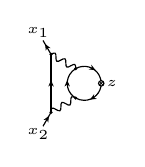
\begin{tikzpicture}[x=0.340cm, y=0.340cm, line width=0.420pt, baseline={([yshift=-0.6ex]0,0)}]
  \draw (-0.625,-1.083) -- (-0.625,1.083);
  \fill (-0.625,0.119) -- (-0.727,-0.119) -- (-0.625,-0.042) -- (-0.523,-0.119) -- cycle;
  \draw (0.297,0.550) arc[start angle=120.000, end angle=0.000, radius=0.635];
  \fill (1.036,0.490) -- (0.880,0.698) -- (0.896,0.571) -- (0.778,0.521) -- cycle;
  \draw (1.250,0.000) arc[start angle=360.000, end angle=240.000, radius=0.635];
  \fill (0.829,-0.610) -- (1.087,-0.579) -- (0.969,-0.529) -- (0.985,-0.402) -- cycle;
  \draw (0.297,-0.550) arc[start angle=240.000, end angle=120.000, radius=0.635];
  \fill (-0.020,0.119) -- (-0.122,-0.119) -- (-0.020,-0.042) -- (0.082,-0.119) -- cycle;
  \draw plot[smooth, tension=0.7] coordinates {(-0.625,1.083) (-0.538,1.126) (-0.475,1.129) (-0.446,1.073) (-0.441,0.976) (-0.435,0.879) (-0.406,0.823) (-0.343,0.826) (-0.256,0.870) (-0.169,0.913) (-0.106,0.916) (-0.077,0.860) (-0.072,0.763) (-0.066,0.666) (-0.037,0.610) (0.026,0.613) (0.113,0.657) (0.200,0.700) (0.263,0.703) (0.292,0.647) (0.297,0.550)};
  \draw plot[smooth, tension=0.7] coordinates {(-0.625,-1.083) (-0.620,-0.985) (-0.590,-0.930) (-0.527,-0.932) (-0.441,-0.976) (-0.354,-1.020) (-0.291,-1.022) (-0.262,-0.967) (-0.256,-0.870) (-0.251,-0.772) (-0.221,-0.717) (-0.158,-0.719) (-0.072,-0.763) (0.015,-0.807) (0.078,-0.809) (0.107,-0.754) (0.113,-0.657) (0.118,-0.559) (0.148,-0.504) (0.211,-0.506) (0.297,-0.550)};
  \draw (-0.625,1.083) -- (-0.925,1.602);
  \fill (-0.850,1.472) -- (-0.819,1.214) -- (-0.769,1.332) -- (-0.642,1.316) -- cycle;
  \draw (-0.625,-1.083) -- (-0.925,-1.602);
  \fill (-0.700,-1.213) -- (-0.908,-1.369) -- (-0.781,-1.353) -- (-0.731,-1.471) -- cycle;
  \draw[fill=white] (1.250,0.000) circle (0.100);
  \draw[line width=0.298pt] (1.320,0.070) -- (1.180,-0.070) (1.320,-0.070) -- (1.180,0.070);
  \fill (-0.625,1.083) circle (0.064);
  \fill (-0.625,-1.083) circle (0.064);
  \fill (0.297,-0.550) circle (0.064);
  \fill (0.297,0.550) circle (0.064);
  \node[font=\tiny, inner sep=0pt, anchor=180] at (1.440,0.000) {$z$};
  \node[font=\tiny, inner sep=0pt, anchor=300] at (-0.970,1.680) {$x_{1}$};
  \node[font=\tiny, inner sep=0pt, anchor=60] at (-0.970,-1.680) {$x_{2}$};
\end{tikzpicture}}
\diagramgap
\mbox{$\displaystyle +\,$\,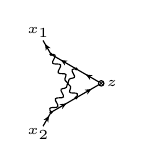
\begin{tikzpicture}[x=0.340cm, y=0.340cm, line width=0.420pt, baseline={([yshift=-0.6ex]0,0)}]
  \draw (0.312,0.541) -- (-0.625,1.083);
  \fill (-0.260,0.872) -- (-0.104,0.664) -- (-0.120,0.791) -- (-0.002,0.841) -- cycle;
  \draw (0.312,-0.541) -- (1.250,0.000);
  \fill (0.885,-0.211) -- (0.627,-0.242) -- (0.745,-0.292) -- (0.729,-0.419) -- cycle;
  \draw (-0.625,-1.083) -- (0.312,-0.541);
  \fill (-0.053,-0.752) -- (-0.311,-0.783) -- (-0.192,-0.833) -- (-0.209,-0.960) -- cycle;
  \draw (1.250,0.000) -- (0.312,0.541);
  \fill (0.678,0.330) -- (0.834,0.123) -- (0.817,0.250) -- (0.936,0.299) -- cycle;
  \draw plot[smooth, tension=0.7] coordinates {(-0.625,1.083) (-0.530,1.077) (-0.475,1.049) (-0.478,0.987) (-0.521,0.902) (-0.564,0.817) (-0.566,0.756) (-0.512,0.727) (-0.417,0.722) (-0.322,0.716) (-0.267,0.688) (-0.270,0.626) (-0.313,0.541) (-0.355,0.456) (-0.358,0.395) (-0.303,0.366) (-0.208,0.361) (-0.114,0.355) (-0.066,0.323) (-0.077,0.256) (-0.104,0.180) (-0.104,0.120) (-0.070,0.080) (-0.030,0.043) (0.000,0.000) (0.030,-0.043) (0.070,-0.080) (0.104,-0.120) (0.104,-0.180) (0.077,-0.256) (0.066,-0.323) (0.114,-0.355) (0.208,-0.361) (0.303,-0.366) (0.358,-0.395) (0.355,-0.456) (0.312,-0.541)};
  \draw plot[smooth, tension=0.7] coordinates {(-0.625,-1.083) (-0.668,-0.998) (-0.670,-0.936) (-0.616,-0.907) (-0.521,-0.902) (-0.426,-0.897) (-0.371,-0.868) (-0.374,-0.807) (-0.417,-0.722) (-0.460,-0.637) (-0.462,-0.575) (-0.407,-0.547) (-0.313,-0.541) (-0.218,-0.536) (-0.163,-0.507) (-0.165,-0.446) (-0.208,-0.361) (-0.251,-0.276) (-0.246,-0.219) (-0.184,-0.195) (-0.104,-0.180) (-0.052,-0.150) (-0.034,-0.101) (-0.022,-0.047) (0.000,0.000) (0.022,0.047) (0.034,0.101) (0.052,0.150) (0.104,0.180) (0.184,0.195) (0.246,0.219) (0.251,0.276) (0.208,0.361) (0.165,0.446) (0.163,0.507) (0.218,0.536) (0.312,0.541)};
  \draw (-0.625,1.083) -- (-0.925,1.602);
  \fill (-0.850,1.472) -- (-0.819,1.214) -- (-0.769,1.332) -- (-0.642,1.316) -- cycle;
  \draw (-0.625,-1.083) -- (-0.925,-1.602);
  \fill (-0.700,-1.213) -- (-0.908,-1.369) -- (-0.781,-1.353) -- (-0.731,-1.471) -- cycle;
  \draw[fill=white] (1.250,0.000) circle (0.100);
  \draw[line width=0.298pt] (1.320,0.070) -- (1.180,-0.070) (1.320,-0.070) -- (1.180,0.070);
  \fill (-0.625,1.083) circle (0.064);
  \fill (-0.625,-1.083) circle (0.064);
  \fill (0.312,-0.541) circle (0.064);
  \fill (0.312,0.541) circle (0.064);
  \node[font=\tiny, inner sep=0pt, anchor=180] at (1.440,0.000) {$z$};
  \node[font=\tiny, inner sep=0pt, anchor=300] at (-0.970,1.680) {$x_{1}$};
  \node[font=\tiny, inner sep=0pt, anchor=60] at (-0.970,-1.680) {$x_{2}$};
\end{tikzpicture}}
\diagramgap
\mbox{$\displaystyle +\,$\,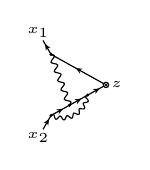
\begin{tikzpicture}[x=0.340cm, y=0.340cm, line width=0.420pt, baseline={([yshift=-0.6ex]0,0)}]
  \draw (1.367,0.000) -- (-0.684,1.141);
  \fill (0.238,0.629) -- (0.397,0.423) -- (0.378,0.550) -- (0.496,0.602) -- cycle;
  \draw (0.684,-0.380) -- (1.367,0.000);
  \fill (1.130,-0.132) -- (0.872,-0.159) -- (0.989,-0.211) -- (0.971,-0.337) -- cycle;
  \draw (-0.684,-1.141) -- (0.000,-0.761);
  \fill (-0.238,-0.893) -- (-0.496,-0.920) -- (-0.378,-0.971) -- (-0.397,-1.098) -- cycle;
  \draw (0.000,-0.761) -- (0.684,-0.380);
  \fill (0.446,-0.513) -- (0.188,-0.540) -- (0.305,-0.591) -- (0.287,-0.718) -- cycle;
  \draw plot[smooth, tension=0.7] coordinates {(-0.684,1.141) (-0.602,1.122) (-0.559,1.088) (-0.571,1.035) (-0.622,0.968) (-0.672,0.901) (-0.684,0.848) (-0.641,0.815) (-0.559,0.795) (-0.478,0.776) (-0.435,0.743) (-0.447,0.689) (-0.497,0.623) (-0.548,0.556) (-0.560,0.502) (-0.517,0.469) (-0.435,0.450) (-0.354,0.430) (-0.311,0.397) (-0.322,0.344) (-0.373,0.277) (-0.423,0.210) (-0.435,0.157) (-0.392,0.123) (-0.311,0.104) (-0.229,0.084) (-0.186,0.051) (-0.198,-0.002) (-0.249,-0.069) (-0.299,-0.136) (-0.311,-0.189) (-0.268,-0.223) (-0.186,-0.242) (-0.105,-0.262) (-0.062,-0.295) (-0.074,-0.348) (-0.124,-0.415) (-0.175,-0.482) (-0.187,-0.535) (-0.144,-0.568) (-0.062,-0.588) (0.019,-0.607) (0.062,-0.641) (0.050,-0.694) (0.000,-0.761)};
  \draw plot[smooth, tension=0.7] coordinates {(-0.684,-1.141) (-0.631,-1.109) (-0.592,-1.101) (-0.569,-1.133) (-0.553,-1.193) (-0.533,-1.253) (-0.501,-1.283) (-0.460,-1.270) (-0.416,-1.225) (-0.374,-1.179) (-0.340,-1.161) (-0.308,-1.184) (-0.275,-1.237) (-0.238,-1.288) (-0.200,-1.308) (-0.164,-1.284) (-0.135,-1.228) (-0.109,-1.171) (-0.081,-1.144) (-0.044,-1.157) (0.003,-1.198) (0.053,-1.237) (0.096,-1.244) (0.123,-1.210) (0.135,-1.148) (0.143,-1.087) (0.162,-1.052) (0.201,-1.054) (0.258,-1.080) (0.317,-1.102) (0.360,-1.097) (0.376,-1.057) (0.370,-0.994) (0.360,-0.933) (0.368,-0.894) (0.406,-0.885) (0.468,-0.893) (0.531,-0.897) (0.570,-0.879) (0.574,-0.836) (0.550,-0.778) (0.522,-0.722) (0.519,-0.683) (0.552,-0.663) (0.614,-0.653) (0.675,-0.638) (0.708,-0.610) (0.699,-0.568) (0.659,-0.519) (0.616,-0.474) (0.602,-0.437) (0.628,-0.408) (0.684,-0.380)};
  \draw (-0.684,1.141) -- (-0.984,1.661);
  \fill (-0.908,1.530) -- (-0.877,1.273) -- (-0.828,1.391) -- (-0.701,1.375) -- cycle;
  \draw (-0.684,-1.141) -- (-0.984,-1.661);
  \fill (-0.759,-1.272) -- (-0.967,-1.427) -- (-0.840,-1.411) -- (-0.790,-1.530) -- cycle;
  \draw[fill=white] (1.367,0.000) circle (0.100);
  \draw[line width=0.298pt] (1.437,0.070) -- (1.297,-0.070) (1.437,-0.070) -- (1.297,0.070);
  \fill (-0.684,1.141) circle (0.064);
  \fill (-0.684,-1.141) circle (0.064);
  \fill (0.000,-0.761) circle (0.064);
  \fill (0.684,-0.380) circle (0.064);
  \node[font=\tiny, inner sep=0pt, anchor=180] at (1.557,0.000) {$z$};
  \node[font=\tiny, inner sep=0pt, anchor=300] at (-1.029,1.739) {$x_{1}$};
  \node[font=\tiny, inner sep=0pt, anchor=60] at (-1.029,-1.739) {$x_{2}$};
\end{tikzpicture}}
\diagramgap
\mbox{$\displaystyle +\,$\,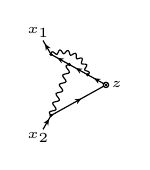
\begin{tikzpicture}[x=0.340cm, y=0.340cm, line width=0.420pt, baseline={([yshift=-0.6ex]0,0)}]
  \draw (0.000,0.761) -- (-0.684,1.141);
  \fill (-0.446,1.009) -- (-0.287,0.804) -- (-0.305,0.931) -- (-0.188,0.982) -- cycle;
  \draw (-0.684,-1.141) -- (1.367,0.000);
  \fill (0.446,-0.513) -- (0.188,-0.540) -- (0.305,-0.591) -- (0.287,-0.718) -- cycle;
  \draw (1.367,0.000) -- (0.684,0.380);
  \fill (0.921,0.248) -- (1.080,0.043) -- (1.062,0.170) -- (1.180,0.221) -- cycle;
  \draw (0.684,0.380) -- (0.000,0.761);
  \fill (0.238,0.629) -- (0.397,0.423) -- (0.378,0.550) -- (0.496,0.602) -- cycle;
  \draw plot[smooth, tension=0.7] coordinates {(-0.684,1.141) (-0.673,1.204) (-0.646,1.238) (-0.604,1.231) (-0.553,1.193) (-0.505,1.153) (-0.468,1.140) (-0.440,1.168) (-0.416,1.225) (-0.387,1.282) (-0.352,1.307) (-0.313,1.288) (-0.275,1.237) (-0.241,1.185) (-0.209,1.162) (-0.175,1.180) (-0.135,1.228) (-0.091,1.273) (-0.050,1.287) (-0.018,1.258) (0.003,1.198) (0.020,1.138) (0.044,1.107) (0.083,1.115) (0.135,1.148) (0.190,1.179) (0.233,1.180) (0.255,1.143) (0.258,1.080) (0.257,1.018) (0.271,0.981) (0.310,0.977) (0.370,0.994) (0.432,1.007) (0.473,0.996) (0.483,0.954) (0.468,0.893) (0.449,0.833) (0.451,0.794) (0.487,0.779) (0.550,0.778) (0.613,0.773) (0.649,0.750) (0.646,0.707) (0.614,0.653) (0.578,0.601) (0.569,0.563) (0.600,0.538) (0.659,0.519) (0.718,0.496) (0.746,0.463) (0.731,0.423) (0.684,0.380)};
  \draw plot[smooth, tension=0.7] coordinates {(-0.684,-1.141) (-0.734,-1.074) (-0.746,-1.021) (-0.703,-0.988) (-0.622,-0.968) (-0.540,-0.949) (-0.497,-0.915) (-0.509,-0.862) (-0.559,-0.795) (-0.610,-0.728) (-0.622,-0.675) (-0.579,-0.642) (-0.497,-0.623) (-0.416,-0.603) (-0.373,-0.570) (-0.385,-0.517) (-0.435,-0.450) (-0.486,-0.383) (-0.497,-0.330) (-0.455,-0.296) (-0.373,-0.277) (-0.291,-0.257) (-0.248,-0.224) (-0.260,-0.171) (-0.311,-0.104) (-0.361,-0.037) (-0.373,0.016) (-0.330,0.050) (-0.249,0.069) (-0.167,0.089) (-0.124,0.122) (-0.136,0.175) (-0.186,0.242) (-0.237,0.309) (-0.249,0.362) (-0.206,0.396) (-0.124,0.415) (-0.043,0.435) (0.000,0.468) (-0.012,0.521) (-0.062,0.588) (-0.113,0.655) (-0.124,0.708) (-0.082,0.741) (0.000,0.761)};
  \draw (-0.684,1.141) -- (-0.984,1.661);
  \fill (-0.908,1.530) -- (-0.877,1.273) -- (-0.828,1.391) -- (-0.701,1.375) -- cycle;
  \draw (-0.684,-1.141) -- (-0.984,-1.661);
  \fill (-0.759,-1.272) -- (-0.967,-1.427) -- (-0.840,-1.411) -- (-0.790,-1.530) -- cycle;
  \draw[fill=white] (1.367,0.000) circle (0.100);
  \draw[line width=0.298pt] (1.437,0.070) -- (1.297,-0.070) (1.437,-0.070) -- (1.297,0.070);
  \fill (-0.684,1.141) circle (0.064);
  \fill (-0.684,-1.141) circle (0.064);
  \fill (0.684,0.380) circle (0.064);
  \fill (0.000,0.761) circle (0.064);
  \node[font=\tiny, inner sep=0pt, anchor=180] at (1.557,0.000) {$z$};
  \node[font=\tiny, inner sep=0pt, anchor=300] at (-1.029,1.739) {$x_{1}$};
  \node[font=\tiny, inner sep=0pt, anchor=60] at (-1.029,-1.739) {$x_{2}$};
\end{tikzpicture}}
\diagramgap
\mbox{$\displaystyle -\,$\,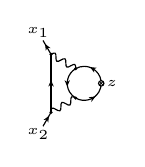
\begin{tikzpicture}[x=0.340cm, y=0.340cm, line width=0.420pt, baseline={([yshift=-0.6ex]0,0)}]
  \draw (-0.625,-1.083) -- (-0.625,1.083);
  \fill (-0.625,0.119) -- (-0.727,-0.119) -- (-0.625,-0.042) -- (-0.523,-0.119) -- cycle;
  \draw (0.297,-0.550) arc[start angle=240.000, end angle=360.000, radius=0.635];
  \fill (1.036,-0.490) -- (0.778,-0.521) -- (0.896,-0.571) -- (0.880,-0.698) -- cycle;
  \draw (1.250,0.000) arc[start angle=360.000, end angle=480.000, radius=0.635];
  \fill (0.829,0.610) -- (0.985,0.402) -- (0.969,0.529) -- (1.087,0.579) -- cycle;
  \draw (0.297,0.550) arc[start angle=120.000, end angle=240.000, radius=0.635];
  \fill (-0.020,-0.119) -- (0.082,0.119) -- (-0.020,0.042) -- (-0.122,0.119) -- cycle;
  \draw plot[smooth, tension=0.7] coordinates {(-0.625,1.083) (-0.538,1.126) (-0.475,1.129) (-0.446,1.073) (-0.441,0.976) (-0.435,0.879) (-0.406,0.823) (-0.343,0.826) (-0.256,0.870) (-0.169,0.913) (-0.106,0.916) (-0.077,0.860) (-0.072,0.763) (-0.066,0.666) (-0.037,0.610) (0.026,0.613) (0.113,0.657) (0.200,0.700) (0.263,0.703) (0.292,0.647) (0.297,0.550)};
  \draw plot[smooth, tension=0.7] coordinates {(-0.625,-1.083) (-0.620,-0.985) (-0.590,-0.930) (-0.527,-0.932) (-0.441,-0.976) (-0.354,-1.020) (-0.291,-1.022) (-0.262,-0.967) (-0.256,-0.870) (-0.251,-0.772) (-0.221,-0.717) (-0.158,-0.719) (-0.072,-0.763) (0.015,-0.807) (0.078,-0.809) (0.107,-0.754) (0.113,-0.657) (0.118,-0.559) (0.148,-0.504) (0.211,-0.506) (0.297,-0.550)};
  \draw (-0.625,1.083) -- (-0.925,1.602);
  \fill (-0.850,1.472) -- (-0.819,1.214) -- (-0.769,1.332) -- (-0.642,1.316) -- cycle;
  \draw (-0.625,-1.083) -- (-0.925,-1.602);
  \fill (-0.700,-1.213) -- (-0.908,-1.369) -- (-0.781,-1.353) -- (-0.731,-1.471) -- cycle;
  \draw[fill=white] (1.250,0.000) circle (0.100);
  \draw[line width=0.298pt] (1.320,0.070) -- (1.180,-0.070) (1.320,-0.070) -- (1.180,0.070);
  \fill (-0.625,1.083) circle (0.064);
  \fill (-0.625,-1.083) circle (0.064);
  \fill (0.297,0.550) circle (0.064);
  \fill (0.297,-0.550) circle (0.064);
  \node[font=\tiny, inner sep=0pt, anchor=180] at (1.440,0.000) {$z$};
  \node[font=\tiny, inner sep=0pt, anchor=300] at (-0.970,1.680) {$x_{1}$};
  \node[font=\tiny, inner sep=0pt, anchor=60] at (-0.970,-1.680) {$x_{2}$};
\end{tikzpicture}}
\diagramgap
\mbox{$\displaystyle -\,$\,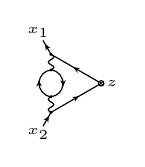
\begin{tikzpicture}[x=0.340cm, y=0.340cm, line width=0.420pt, baseline={([yshift=-0.6ex]0,0)}]
  \draw (1.250,0.000) -- (-0.625,1.083);
  \fill (0.209,0.601) -- (0.365,0.393) -- (0.349,0.520) -- (0.467,0.570) -- cycle;
  \draw (-0.625,-1.083) -- (1.250,0.000);
  \fill (0.416,-0.482) -- (0.158,-0.513) -- (0.276,-0.562) -- (0.260,-0.689) -- cycle;
  \draw (-0.625,-0.500) arc[start angle=263.974, end angle=96.026, radius=0.503];
  \fill (-1.075,0.119) -- (-1.177,-0.119) -- (-1.075,-0.042) -- (-0.973,-0.119) -- cycle;
  \draw (-0.625,0.500) arc[start angle=83.974, end angle=-83.974, radius=0.503];
  \fill (-0.175,-0.119) -- (-0.073,0.119) -- (-0.175,0.042) -- (-0.277,0.119) -- cycle;
  \draw plot[smooth, tension=0.7] coordinates {(-0.625,1.083) (-0.551,1.034) (-0.520,0.985) (-0.551,0.937) (-0.625,0.888) (-0.699,0.840) (-0.730,0.791) (-0.699,0.743) (-0.625,0.694) (-0.551,0.646) (-0.520,0.597) (-0.551,0.549) (-0.625,0.500)};
  \draw plot[smooth, tension=0.7] coordinates {(-0.625,-1.083) (-0.699,-1.034) (-0.730,-0.985) (-0.699,-0.937) (-0.625,-0.888) (-0.551,-0.840) (-0.520,-0.791) (-0.551,-0.743) (-0.625,-0.694) (-0.699,-0.646) (-0.730,-0.597) (-0.699,-0.549) (-0.625,-0.500)};
  \draw (-0.625,1.083) -- (-0.925,1.602);
  \fill (-0.850,1.472) -- (-0.819,1.214) -- (-0.769,1.332) -- (-0.642,1.316) -- cycle;
  \draw (-0.625,-1.083) -- (-0.925,-1.602);
  \fill (-0.700,-1.213) -- (-0.908,-1.369) -- (-0.781,-1.353) -- (-0.731,-1.471) -- cycle;
  \draw[fill=white] (1.250,0.000) circle (0.100);
  \draw[line width=0.298pt] (1.320,0.070) -- (1.180,-0.070) (1.320,-0.070) -- (1.180,0.070);
  \fill (-0.625,1.083) circle (0.064);
  \fill (-0.625,-1.083) circle (0.064);
  \fill (-0.625,0.500) circle (0.064);
  \fill (-0.625,-0.500) circle (0.064);
  \node[font=\tiny, inner sep=0pt, anchor=180] at (1.440,0.000) {$z$};
  \node[font=\tiny, inner sep=0pt, anchor=300] at (-0.970,1.680) {$x_{1}$};
  \node[font=\tiny, inner sep=0pt, anchor=60] at (-0.970,-1.680) {$x_{2}$};
\end{tikzpicture}}
\diagramgap
\mbox{$\displaystyle +\,$\,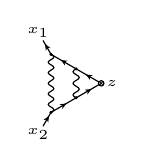
\begin{tikzpicture}[x=0.340cm, y=0.340cm, line width=0.420pt, baseline={([yshift=-0.6ex]0,0)}]
  \draw (0.312,0.541) -- (-0.625,1.083);
  \fill (-0.260,0.872) -- (-0.104,0.664) -- (-0.120,0.791) -- (-0.002,0.841) -- cycle;
  \draw (0.312,-0.541) -- (1.250,0.000);
  \fill (0.885,-0.211) -- (0.627,-0.242) -- (0.745,-0.292) -- (0.729,-0.419) -- cycle;
  \draw (-0.625,-1.083) -- (0.312,-0.541);
  \fill (-0.053,-0.752) -- (-0.311,-0.783) -- (-0.192,-0.833) -- (-0.209,-0.960) -- cycle;
  \draw (1.250,0.000) -- (0.312,0.541);
  \fill (0.678,0.330) -- (0.834,0.123) -- (0.817,0.250) -- (0.936,0.299) -- cycle;
  \draw plot[smooth, tension=0.7] coordinates {(-0.625,1.083) (-0.550,1.033) (-0.519,0.984) (-0.550,0.935) (-0.625,0.886) (-0.700,0.837) (-0.731,0.787) (-0.700,0.738) (-0.625,0.689) (-0.550,0.640) (-0.519,0.590) (-0.550,0.541) (-0.625,0.492) (-0.700,0.443) (-0.731,0.394) (-0.700,0.344) (-0.625,0.295) (-0.550,0.246) (-0.519,0.197) (-0.550,0.148) (-0.625,0.098) (-0.700,0.049) (-0.731,0.000) (-0.700,-0.049) (-0.625,-0.098) (-0.550,-0.148) (-0.519,-0.197) (-0.550,-0.246) (-0.625,-0.295) (-0.700,-0.344) (-0.731,-0.394) (-0.700,-0.443) (-0.625,-0.492) (-0.550,-0.541) (-0.519,-0.590) (-0.550,-0.640) (-0.625,-0.689) (-0.700,-0.738) (-0.731,-0.787) (-0.700,-0.837) (-0.625,-0.886) (-0.550,-0.935) (-0.519,-0.984) (-0.550,-1.033) (-0.625,-1.083)};
  \draw plot[smooth, tension=0.7] coordinates {(0.312,-0.541) (0.230,-0.487) (0.196,-0.433) (0.230,-0.379) (0.312,-0.325) (0.395,-0.271) (0.429,-0.217) (0.395,-0.162) (0.312,-0.108) (0.230,-0.054) (0.196,0.000) (0.230,0.054) (0.312,0.108) (0.395,0.162) (0.429,0.217) (0.395,0.271) (0.312,0.325) (0.230,0.379) (0.196,0.433) (0.230,0.487) (0.312,0.541)};
  \draw (-0.625,1.083) -- (-0.925,1.602);
  \fill (-0.850,1.472) -- (-0.819,1.214) -- (-0.769,1.332) -- (-0.642,1.316) -- cycle;
  \draw (-0.625,-1.083) -- (-0.925,-1.602);
  \fill (-0.700,-1.213) -- (-0.908,-1.369) -- (-0.781,-1.353) -- (-0.731,-1.471) -- cycle;
  \draw[fill=white] (1.250,0.000) circle (0.100);
  \draw[line width=0.298pt] (1.320,0.070) -- (1.180,-0.070) (1.320,-0.070) -- (1.180,0.070);
  \fill (-0.625,1.083) circle (0.064);
  \fill (-0.625,-1.083) circle (0.064);
  \fill (0.312,-0.541) circle (0.064);
  \fill (0.312,0.541) circle (0.064);
  \node[font=\tiny, inner sep=0pt, anchor=180] at (1.440,0.000) {$z$};
  \node[font=\tiny, inner sep=0pt, anchor=300] at (-0.970,1.680) {$x_{1}$};
  \node[font=\tiny, inner sep=0pt, anchor=60] at (-0.970,-1.680) {$x_{2}$};
\end{tikzpicture}}
\diagramgap
\mbox{$\displaystyle -\,$\,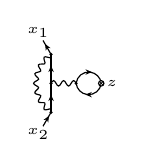
\begin{tikzpicture}[x=0.340cm, y=0.340cm, line width=0.420pt, baseline={([yshift=-0.6ex]0,0)}]
  \draw (-0.625,0.000) -- (-0.625,1.083);
  \fill (-0.625,0.661) -- (-0.727,0.422) -- (-0.625,0.499) -- (-0.523,0.422) -- cycle;
  \draw (0.312,0.000) arc[start angle=173.974, end angle=6.026, radius=0.471];
  \fill (0.901,0.422) -- (0.662,0.524) -- (0.739,0.422) -- (0.662,0.320) -- cycle;
  \draw (1.250,0.000) arc[start angle=353.974, end angle=186.026, radius=0.471];
  \fill (0.662,-0.422) -- (0.901,-0.524) -- (0.823,-0.422) -- (0.901,-0.320) -- cycle;
  \draw (-0.625,-1.083) -- (-0.625,0.000);
  \fill (-0.625,-0.422) -- (-0.727,-0.661) -- (-0.625,-0.583) -- (-0.523,-0.661) -- cycle;
  \draw plot[smooth, tension=0.7] coordinates {(-0.625,1.083) (-0.622,1.008) (-0.638,0.963) (-0.685,0.958) (-0.757,0.977) (-0.831,0.992) (-0.881,0.979) (-0.892,0.929) (-0.874,0.855) (-0.852,0.784) (-0.856,0.737) (-0.900,0.719) (-0.975,0.720) (-1.051,0.716) (-1.095,0.690) (-1.094,0.639) (-1.058,0.572) (-1.018,0.509) (-1.010,0.462) (-1.049,0.434) (-1.121,0.416) (-1.193,0.393) (-1.230,0.357) (-1.216,0.307) (-1.164,0.252) (-1.110,0.201) (-1.090,0.157) (-1.120,0.121) (-1.185,0.084) (-1.249,0.044) (-1.276,0.000) (-1.249,-0.044) (-1.185,-0.084) (-1.120,-0.121) (-1.090,-0.157) (-1.110,-0.201) (-1.164,-0.252) (-1.216,-0.307) (-1.230,-0.357) (-1.193,-0.393) (-1.121,-0.416) (-1.049,-0.434) (-1.010,-0.462) (-1.018,-0.509) (-1.058,-0.572) (-1.094,-0.639) (-1.095,-0.690) (-1.051,-0.716) (-0.975,-0.720) (-0.900,-0.719) (-0.856,-0.737) (-0.852,-0.784) (-0.874,-0.855) (-0.892,-0.929) (-0.881,-0.979) (-0.831,-0.992) (-0.757,-0.977) (-0.685,-0.958) (-0.638,-0.963) (-0.622,-1.008) (-0.625,-1.083)};
  \draw plot[smooth, tension=0.7] coordinates {(-0.625,0.000) (-0.578,0.072) (-0.531,0.101) (-0.484,0.072) (-0.438,0.000) (-0.391,-0.072) (-0.344,-0.101) (-0.297,-0.072) (-0.250,0.000) (-0.203,0.072) (-0.156,0.101) (-0.109,0.072) (-0.063,0.000) (-0.016,-0.072) (0.031,-0.101) (0.078,-0.072) (0.125,0.000) (0.172,0.072) (0.219,0.101) (0.266,0.072) (0.312,0.000)};
  \draw (-0.625,1.083) -- (-0.925,1.602);
  \fill (-0.850,1.472) -- (-0.819,1.214) -- (-0.769,1.332) -- (-0.642,1.316) -- cycle;
  \draw (-0.625,-1.083) -- (-0.925,-1.602);
  \fill (-0.700,-1.213) -- (-0.908,-1.369) -- (-0.781,-1.353) -- (-0.731,-1.471) -- cycle;
  \draw[fill=white] (1.250,0.000) circle (0.100);
  \draw[line width=0.298pt] (1.320,0.070) -- (1.180,-0.070) (1.320,-0.070) -- (1.180,0.070);
  \fill (-0.625,1.083) circle (0.064);
  \fill (-0.625,-1.083) circle (0.064);
  \fill (-0.625,0.000) circle (0.064);
  \fill (0.312,0.000) circle (0.064);
  \node[font=\tiny, inner sep=0pt, anchor=180] at (1.440,0.000) {$z$};
  \node[font=\tiny, inner sep=0pt, anchor=300] at (-0.970,1.680) {$x_{1}$};
  \node[font=\tiny, inner sep=0pt, anchor=60] at (-0.970,-1.680) {$x_{2}$};
\end{tikzpicture}}
\diagramgap
\mbox{$\displaystyle -\,$\,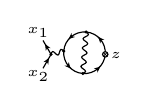
\begin{tikzpicture}[x=0.340cm, y=0.340cm, line width=0.420pt, baseline={([yshift=-0.6ex]0,0)}]
  \draw (0.514,-0.715) arc[start angle=265.551, end angle=355.551, radius=0.778];
  \fill (1.171,-0.453) -- (0.923,-0.531) -- (1.048,-0.558) -- (1.056,-0.686) -- cycle;
  \draw (1.350,0.000) arc[start angle=355.551, end angle=445.551, radius=0.778];
  \fill (1.088,0.657) -- (1.166,0.409) -- (1.193,0.534) -- (1.321,0.542) -- cycle;
  \draw (-0.201,0.121) arc[start angle=175.551, end angle=265.551, radius=0.778];
  \fill (0.061,-0.536) -- (-0.017,-0.288) -- (-0.044,-0.414) -- (-0.172,-0.421) -- cycle;
  \draw (0.635,0.836) arc[start angle=85.551, end angle=175.551, radius=0.778];
  \fill (-0.022,0.574) -- (0.226,0.651) -- (0.101,0.679) -- (0.093,0.806) -- cycle;
  \draw plot[smooth, tension=0.7] coordinates {(-0.675,0.000) (-0.651,0.070) (-0.618,0.105) (-0.572,0.091) (-0.517,0.040) (-0.462,-0.010) (-0.416,-0.025) (-0.383,0.010) (-0.359,0.080) (-0.335,0.151) (-0.302,0.186) (-0.256,0.171) (-0.201,0.121)};
  \draw plot[smooth, tension=0.7] coordinates {(0.635,0.836) (0.697,0.788) (0.721,0.742) (0.691,0.701) (0.621,0.663) (0.552,0.626) (0.522,0.585) (0.546,0.539) (0.608,0.491) (0.670,0.443) (0.694,0.398) (0.664,0.357) (0.595,0.319) (0.525,0.281) (0.495,0.240) (0.519,0.195) (0.581,0.147) (0.644,0.098) (0.668,0.053) (0.637,0.012) (0.568,-0.026) (0.499,-0.064) (0.468,-0.105) (0.492,-0.150) (0.554,-0.198) (0.617,-0.246) (0.641,-0.292) (0.610,-0.333) (0.541,-0.370) (0.472,-0.408) (0.441,-0.449) (0.465,-0.495) (0.528,-0.543) (0.590,-0.591) (0.614,-0.636) (0.583,-0.677) (0.514,-0.715)};
  \draw (-0.675,0.000) -- (-0.975,0.520);
  \fill (-0.900,0.389) -- (-0.869,0.131) -- (-0.819,0.250) -- (-0.692,0.233) -- cycle;
  \draw (-0.675,0.000) -- (-0.975,-0.520);
  \fill (-0.750,-0.130) -- (-0.958,-0.286) -- (-0.831,-0.270) -- (-0.781,-0.388) -- cycle;
  \draw[fill=white] (1.350,0.000) circle (0.100);
  \draw[line width=0.298pt] (1.420,0.070) -- (1.280,-0.070) (1.420,-0.070) -- (1.280,0.070);
  \fill (-0.675,0.000) circle (0.064);
  \fill (0.635,0.836) circle (0.064);
  \fill (0.514,-0.715) circle (0.064);
  \fill (-0.201,0.121) circle (0.064);
  \node[font=\tiny, inner sep=0pt, anchor=176] at (1.539,-0.015) {$z$};
  \node[font=\tiny, inner sep=0pt, anchor=300] at (-1.020,0.598) {$x_{1}$};
  \node[font=\tiny, inner sep=0pt, anchor=60] at (-1.020,-0.598) {$x_{2}$};
\end{tikzpicture}}
\diagramgap
\mbox{$\displaystyle +\,$\,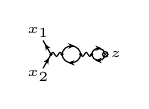
\begin{tikzpicture}[x=0.340cm, y=0.340cm, line width=0.420pt, baseline={([yshift=-0.6ex]0,0)}]
  \draw (0.844,0.000) arc[start angle=173.974, end angle=6.026, radius=0.255];
  \fill (1.216,0.228) -- (0.977,0.330) -- (1.055,0.228) -- (0.977,0.126) -- cycle;
  \draw (1.350,0.000) arc[start angle=353.974, end angle=186.026, radius=0.255];
  \fill (0.977,-0.228) -- (1.216,-0.330) -- (1.139,-0.228) -- (1.216,-0.126) -- cycle;
  \draw (0.434,0.000) arc[start angle=353.974, end angle=186.026, radius=0.352];
  \fill (-0.035,-0.315) -- (0.204,-0.417) -- (0.126,-0.315) -- (0.204,-0.213) -- cycle;
  \draw (-0.266,0.000) arc[start angle=173.974, end angle=6.026, radius=0.352];
  \fill (0.204,0.315) -- (-0.035,0.417) -- (0.043,0.315) -- (-0.035,0.213) -- cycle;
  \draw plot[smooth, tension=0.7] coordinates {(-0.675,0.000) (-0.641,0.052) (-0.607,0.074) (-0.573,0.052) (-0.539,0.000) (-0.504,-0.052) (-0.470,-0.074) (-0.436,-0.052) (-0.402,0.000) (-0.368,0.052) (-0.334,0.074) (-0.300,0.052) (-0.266,0.000)};
  \draw plot[smooth, tension=0.7] coordinates {(0.844,0.000) (0.810,-0.052) (0.776,-0.074) (0.741,-0.052) (0.707,0.000) (0.673,0.052) (0.639,0.074) (0.605,0.052) (0.571,0.000) (0.537,-0.052) (0.503,-0.074) (0.468,-0.052) (0.434,0.000)};
  \draw (-0.675,0.000) -- (-0.975,0.520);
  \fill (-0.900,0.389) -- (-0.869,0.131) -- (-0.819,0.250) -- (-0.692,0.233) -- cycle;
  \draw (-0.675,0.000) -- (-0.975,-0.520);
  \fill (-0.750,-0.130) -- (-0.958,-0.286) -- (-0.831,-0.270) -- (-0.781,-0.388) -- cycle;
  \draw[fill=white] (1.350,0.000) circle (0.100);
  \draw[line width=0.298pt] (1.420,0.070) -- (1.280,-0.070) (1.420,-0.070) -- (1.280,0.070);
  \fill (-0.675,0.000) circle (0.064);
  \fill (0.844,0.000) circle (0.064);
  \fill (-0.266,0.000) circle (0.064);
  \fill (0.434,0.000) circle (0.064);
  \node[font=\tiny, inner sep=0pt, anchor=180] at (1.540,0.000) {$z$};
  \node[font=\tiny, inner sep=0pt, anchor=300] at (-1.020,0.598) {$x_{1}$};
  \node[font=\tiny, inner sep=0pt, anchor=60] at (-1.020,-0.598) {$x_{2}$};
\end{tikzpicture}}
